%%
%% This is file `sample-sigconf.tex',
%% generated with the docstrip utility.
%%
%% The original source files were:
%%
%% samples.dtx  (with options: `sigconf')
%%
%% IMPORTANT NOTICE:
%%
%% For the copyright see the source file.
%%
%% Any modified versions of this file must be renamed
%% with new filenames distinct from sample-sigconf.tex.
%%
%% For distribution of the original source see the terms
%% for copying and modification in the file samples.dtx.
%%
%% This generated file may be distributed as long as the
%% original source files, as listed above, are part of the
%% same distribution. (The sources need not necessarily be
%% in the same archive or directory.)
%%
%% The first command in your LaTeX source must be the \documentclass command.
\documentclass[sigconf,10pt]{acmart}

\settopmatter{printfolios=true}


\providecommand{\tightlist}{%
  \setlength{\itemsep}{0pt}\setlength{\parskip}{0pt}}

%%
%% \BibTeX command to typeset BibTeX logo in the docs
\AtBeginDocument{%
  \providecommand\BibTeX{{%
    \normalfont B\kern-0.5em{\scshape i\kern-0.25em b}\kern-0.8em\TeX}}}

%% Rights management information.  This information is sent to you
%% when you complete the rights form.  These commands have SAMPLE
%% values in them; it is your responsibility as an author to replace
%% the commands and values with those provided to you when you
%% complete the rights form.


%%
%% Submission ID.
%% Use this when submitting an article to a sponsored event. You'll
%% receive a unique submission ID from the organizers
%% of the event, and this ID should be used as the parameter to this command.
%%\acmSubmissionID{123-A56-BU3}

%%
%% The majority of ACM publications use numbered citations and
%% references.  The command \citestyle{authoryear} switches to the
%% "author year" style.
%%
%% If you are preparing content for an event
%% sponsored by ACM SIGGRAPH, you must use the "author year" style of
%% citations and references.
%% Uncommenting
%% the next command will enable that style.
%%\citestyle{acmauthoryear}

%%
%% end of the preamble, start of the body of the document source.
\begin{document}

%%
%% The "title" command has an optional parameter,
%% allowing the author to define a "short title" to be used in page headers.
\title{Towards End-user Web Scraping For Customization}

%%
%% The "author" command and its associated commands are used to define
%% the authors and their affiliations.
%% Of note is the shared affiliation of the first two authors, and the
%% "authornote" and "authornotemark" commands
%% used to denote shared contribution to the research.

\author{Kapaya Katongo}
\affiliation{%
  \institution{MIT CSAIL}
  \city{Cambridge, MA}
  \country{USA}
}
\email{kkatongo@mit.edu}

\author{Geoffrey Litt}
\affiliation{%
  \institution{MIT CSAIL}
  \city{Cambridge, MA}
  \country{USA}
}
\email{glitt@mit.edu}

\author{Daniel Jackson}
\affiliation{%
  \institution{MIT CSAIL}
  \city{Cambridge, MA}
  \country{USA}
}
\email{dnj@csail.mit.edu}

%%
%% By default, the full list of authors will be used in the page
%% headers. Often, this list is too long, and will overlap
%% other information printed in the page headers. This command allows
%% the author to define a more concise list
%% of authors' names for this purpose.
% \renewcommand{\shortauthors}{Trovato and Tobin, et al.}

%%
%% The abstract is a short summary of the work to be presented in the
%% article.
\begin{abstract}
  Websites are malleable: users can run code in the browser to customize
  them. However, this malleability is typically only accessible to
  programmers with knowledge of HTML and Javascript. Previously, we
  developed a tool called Wildcard which empowers end-users to customize
  websites through a data table interface without doing traditional
  programming. However, there is a limit on end-user flexibility with
  Wildcard, because programmers need to create site-specific adapters
  mapping website data to a table view. This means that end-users can
  only customize a website if a programmer has written an adapter for
  it, and cannot extend or repair existing adapters.

  In this paper, we extend Wildcard with a new system for \emph{end-user
  web scraping for customization}. It enables end-users to create,
  extend and repair adapters, by performing concrete demonstrations of
  how the webpage UI maps to a data table. We describe three design
  principles that guided our system's development and are applicable to
  other end-user web scraping and customization systems: (a) users
  should be able to scrape data and use it in a single, unified
  environment, (b) users should be able to extend and repair the
  programs that scrape data via demonstration and (c) users should
  receive live feedback during their demonstrations.

  We have successfully used our system to create, extend and repair
  adapters by demonstration on a variety of websites and we provide
  example usage scenarios that showcase each of our design principles.
\end{abstract}

%%
%% The code below is generated by the tool at http://dl.acm.org/ccs.cfm.
%% Please copy and paste the code instead of the example below.
%%
%% From HERE
\begin{CCSXML}
<ccs2012>
<concept>
<concept_id>10011007.10011006.10011066.10011069</concept_id>
<concept_desc>Software and its engineering~Integrated and visual development environments</concept_desc>
<concept_significance>500</concept_significance>
</concept>
</ccs2012>
\end{CCSXML}

\ccsdesc[500]{Software and its engineering~Integrated and visual development environments}
% To HERE

%%
%% Keywords. The author(s) should pick words that accurately describe
%% the work being presented. Separate the keywords with commas.
\keywords{end-user programming, software customization, web scraping, programming by example}

%% A "teaser" image appears between the author and affiliation
%% information and the body of the document, and typically spans the
%% page.
%\begin{teaserfigure}
%  \includegraphics[width=\textwidth]{sampleteaser}
%  \caption{Seattle Mariners at Spring Training, 2010.}
%  \Description{Enjoying the baseball game from the third-base
%  seats. Ichiro Suzuki preparing to bat.}
%  \label{fig:teaser}
%\end{teaserfigure}

%%
%% This command processes the author and affiliation and title
%% information and builds the first part of the formatted document.
\maketitle

\hypertarget{sec:introduction}{%
\section{Introduction}\label{sec:introduction}}

Many websites on the internet do not meet the exact needs of all of
their users. End-user web customization systems like Chickenfoot
\citep{bolin2005}, Thresher \citep{hogue2005}, Sifter \citep{huynh2006}
and Vegemite \citep{lin2009} help users tweak and adapt websites to fit
their unique requirements, ranging from reorganizing or annotating
content on the website to automating common tasks. In our prior work, we
presented Wildcard \citep{litt2020a}, a customization system which
enables end-users to customize websites through direct manipulation. It
does this by augmenting websites with a table view that shows their
underlying structured data. The table is bidirectionally synchronized
with the original website, so end-users can easily customize the website
by interacting with the table, including sorting and filtering data,
adding annotations, and running computations in a spreadsheet formula
language.

Wildcard has a key limitation. In order to enable end-users to customize
a website, a programmer first needs to code a Javascript adapter that
specifies how to scrape the website content and set up a bidirectional
synchronization with Wildcard's table view. Even though programmers can
share adapters with end-users, this means that an end-user can only use
Wildcard on websites where some programmer has already written an
adapter. Additionally, if an adapter doesn't scrape the desired data, or
stops functioning correctly when a website changes, an end-user has no
recourse to extend or repair it on their own.

\begin{figure*}
  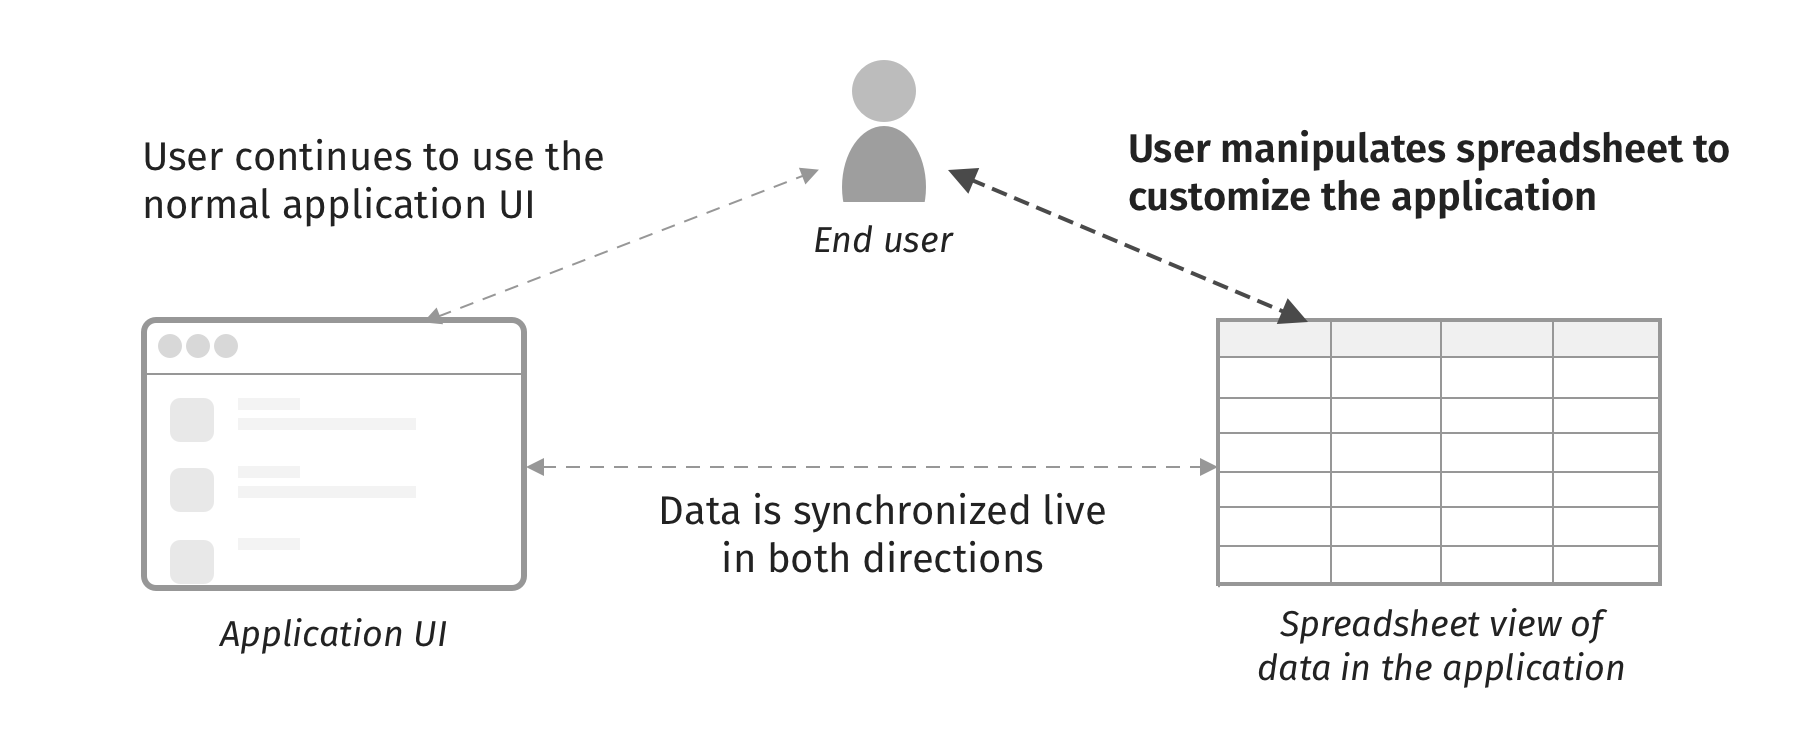
\includegraphics[width=\textwidth]{media/overview.png}
  \caption{\label{fig:overview}Our work enables end-users to create Wildcard site adapters by demonstration.}
\end{figure*}

In this paper, we describe an addition to Wildcard: a system that
enables end-users to create, extend and repair website adapters by
demonstration within the browser. Using this scraping system, an
end-user can perform web customizations using Wildcard on arbitrary
websites, without ever needing to code an adapter. Through a series of
examples, we show that our system can create Wildcard adapters on a
variety of websites via demonstration (Section~\ref{sec:demos}). We also
describe key aspects of our system and how web scraping for
customization leads to a constraint that simplifies the \emph{wrapper
induction} \citep{kushmerick2000} task used to generalize user
demonstrations (Section~\ref{sec:implementation}).

Our key contribution is a set of three design principles that guided the
development of our system, which also offer insights that might be
applied to other end-user web scraping and customization tools
(Section~\ref{sec:design-principles}):

\begin{itemize}
\tightlist
\item
  \textbf{Unified Environment}: Users should be able to scrape data and
  interact with the scraped data in a single, unified environment. This
  minimizes the barrier to fluidly switching back and forth between the
  two tasks, rather than treating them as entirely independent tasks.
\item
  \textbf{Editing By Demonstration}: Users should be able to not only
  create programs for scraping data by demonstration, but also extend
  and repair the programs by demonstration. This enables users to build
  on other users' work, and is especially important in the context of
  web scraping since scrapers break as the underlying website changes.
\item
  \textbf{Live Programming}: Users should receive live feedback as they
  perform demonstrations. The system should indicate how it is
  generalizing from the user's example and what the resulting data will
  look like, so that the user can adjust their demonstrations on the fly
  and quickly arrive at the desired result.
\end{itemize}

Finally, we share our broader vision for web scraping for customization,
and some opportunities for future work, including a proposal for how
Wildcard's spreadsheet-like formula language might augment
demonstrations to provide end-users with more expressiveness in the web
scraping process (Section~\ref{sec:conclusion}).

\hypertarget{sec:demos}{%
\section{Motivating Examples}\label{sec:demos}}

In this section, we show how end-users can create, extend and repair
adapters for Wildcard via demonstration.{ These demos are best viewed as
videos in the online version of this paper
(\url{https://kapaya.github.io/px21}).}

\hypertarget{creating-an-adapter}{%
\subsection{Creating An Adapter}\label{creating-an-adapter}}

Jen wants to customize her experience on Weather.com by sorting the
ten-day forecast based on the description of the weather on each day,
allowing her to easily view all the sunny days. She starts the adapter
creation process by clicking a context menu item within the Weather.com
page, and hovers over a data value she might like to scrape.

\begin{figure*}
  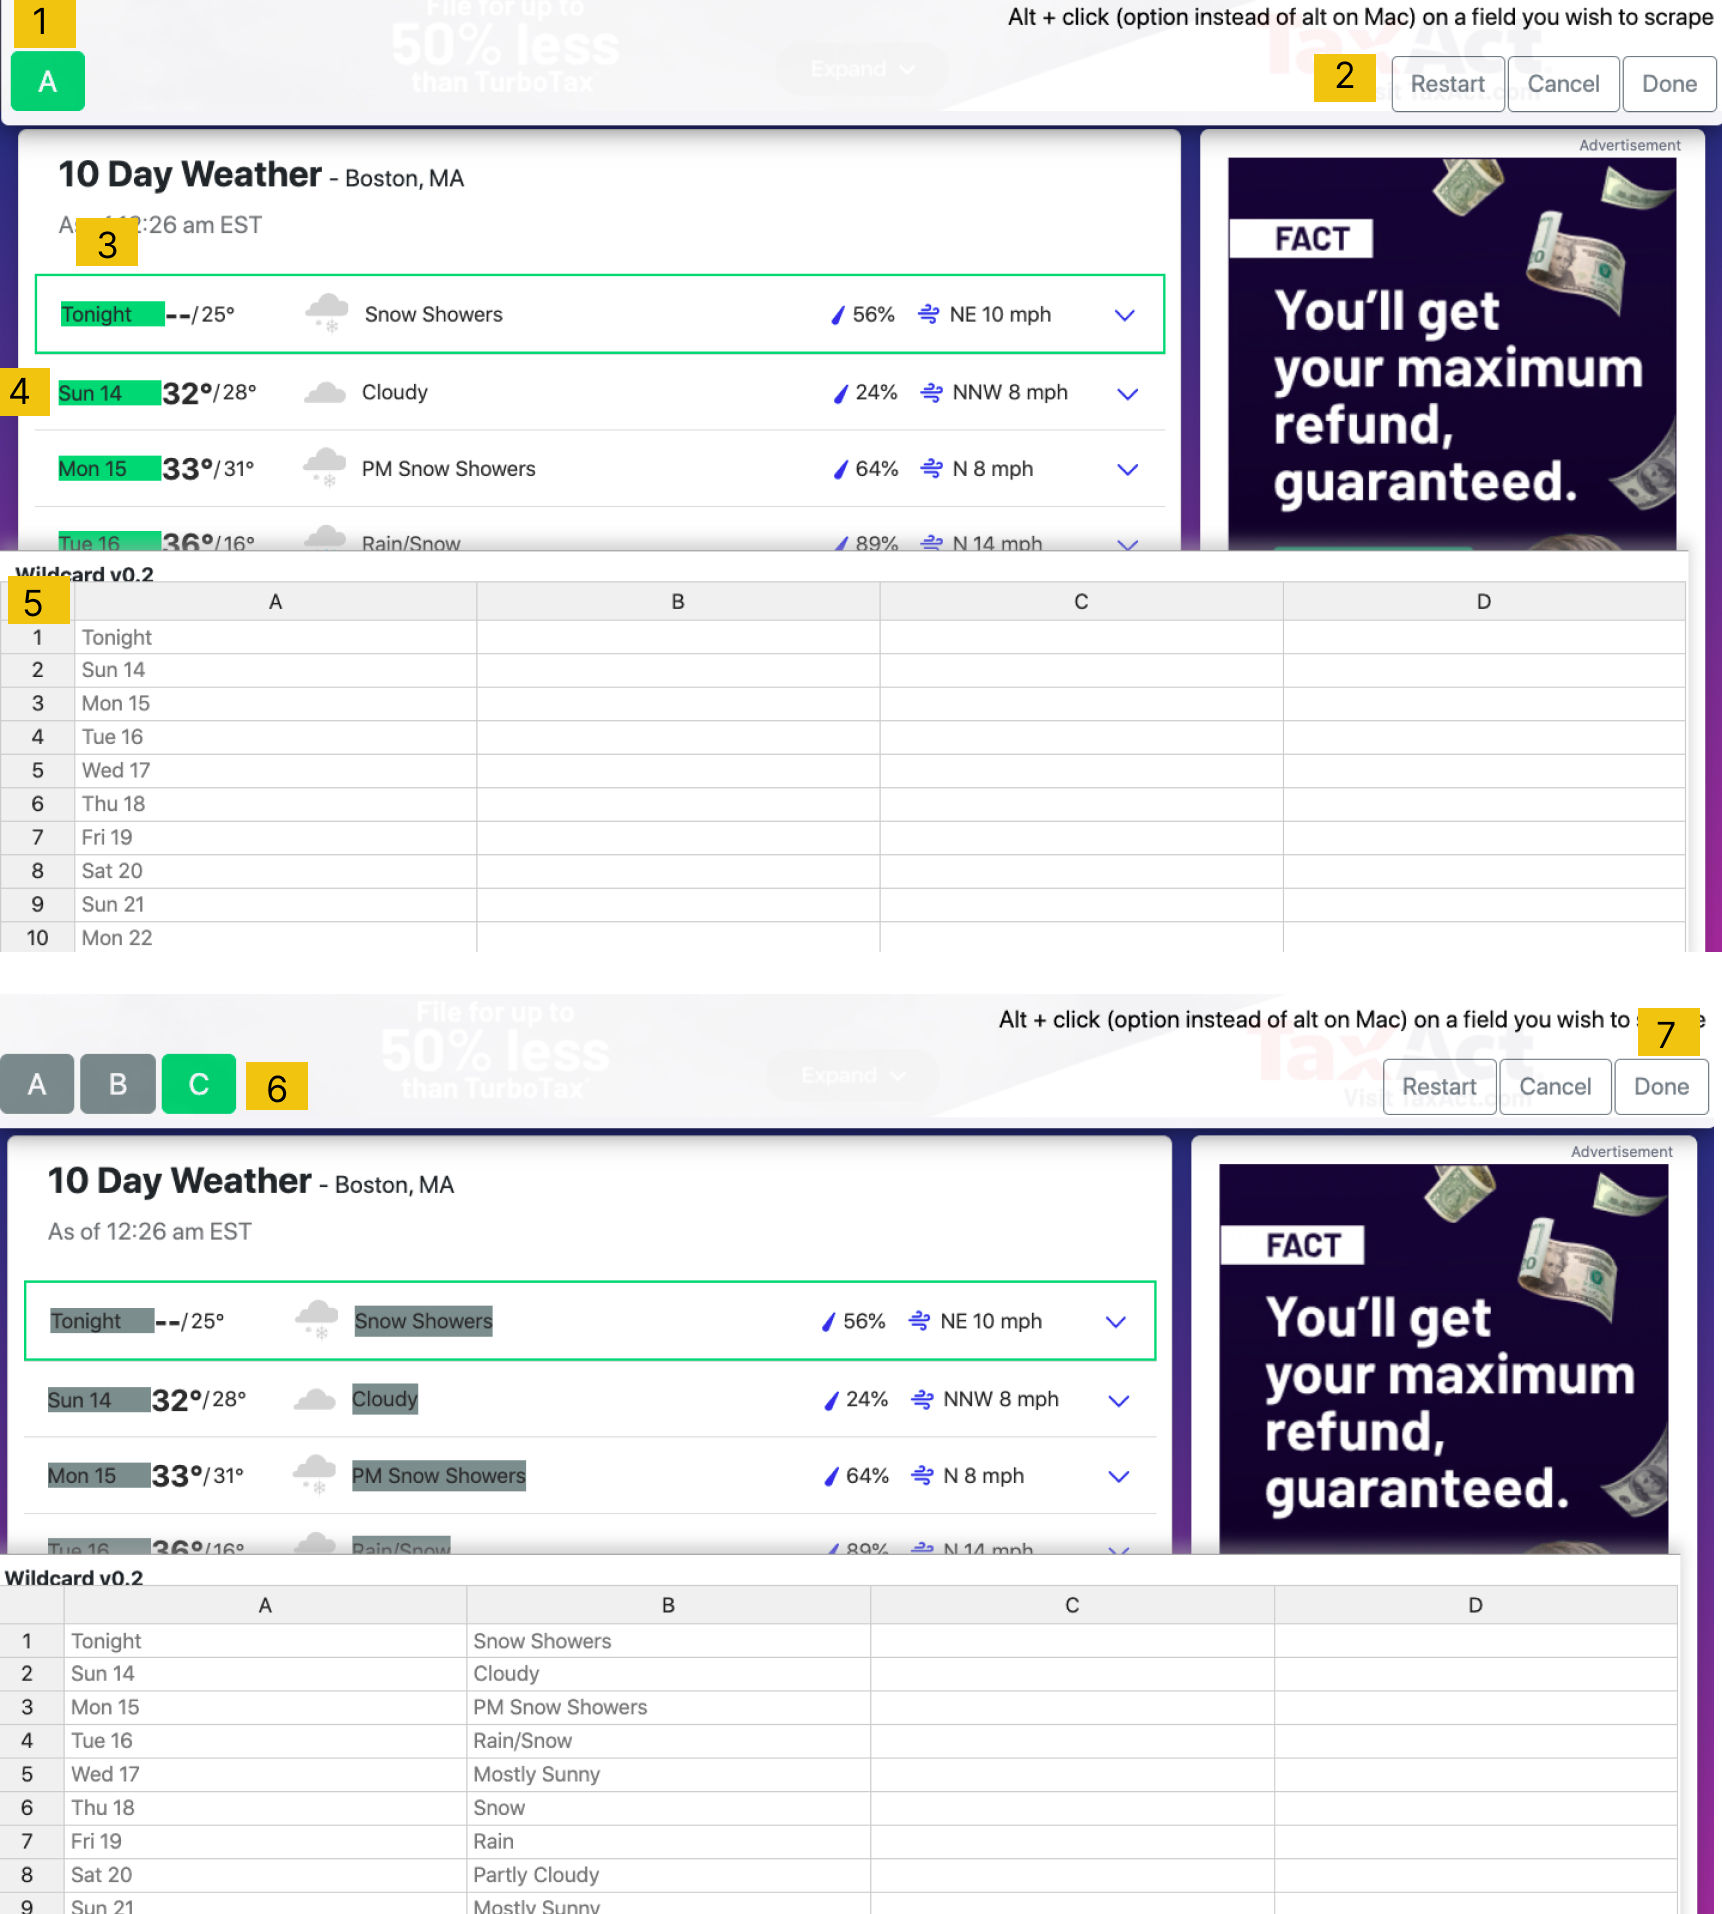
\includegraphics[width=\textwidth]{media/creating.png}
  \caption{\label{fig:creating} Creating an adapter: 1) column data will be scraped into, 2) system's controls, 3) demonstrated column value and row from which columns should be demonstrated from 4) column values determined by generalization algorithm 5) column values populated in table, 6) next column to scrape data into and 7) button to save adapter created by demonstration}
\end{figure*}

The system provides live feedback as Jen hovers, demonstrating the
\textbf{live programming} principle. The workflow steps are shown in
Figure~\ref{fig:creating}:

\begin{itemize}
\tightlist
\item
  The selected row of data is annotated in the page with a border, to
  indicate that she will be demonstrating values from within that row
  (Part 3).
\item
  The selected column of data is highlighted in the page with a green
  background, to show how the system has generalized her demonstration
  across all the rows in the data (Part 4).
\item
  A table view appears at the bottom of the screen, and displays how the
  values will appear in the data table (Part 5).
\end{itemize}

Jen tries hovering over several other elements in the page, taking
advantage of the live feedback environment to decide what data would be
useful. After considering several options, she decides to save the date
field in the first column of the table, and commits the action by
clicking.

Next, she performs a similar process to fill the next column with the
weather descriptions. After filling both columns, she also tries
hovering over previously scraped data, and the toolbar at the top of the
page indicates which column corresponds to the previously scraped data.
Finally, she ends the adapter creation process (Part 7) and is able to
immediately sort the forecast by the weather description column, because
Wildcard provides a \textbf{unified environment} that combines both
scraping and customizing.

\hypertarget{extending-an-adapter}{%
\subsection{Extending An Adapter}\label{extending-an-adapter}}

Jen has previously used Wildcard to customize timeanddate.com, sorting
holidays by day of the week. She comes up with a new customization idea:
sorting holidays by category so she can view all the federal holidays
together. The current site adapter she is using does not populate the
category column in the table, so she needs to extend the adapter. She
can immediately perform the extension in the context of the page, using
our system's support for \textbf{editing by demonstration}.

\begin{figure*}
  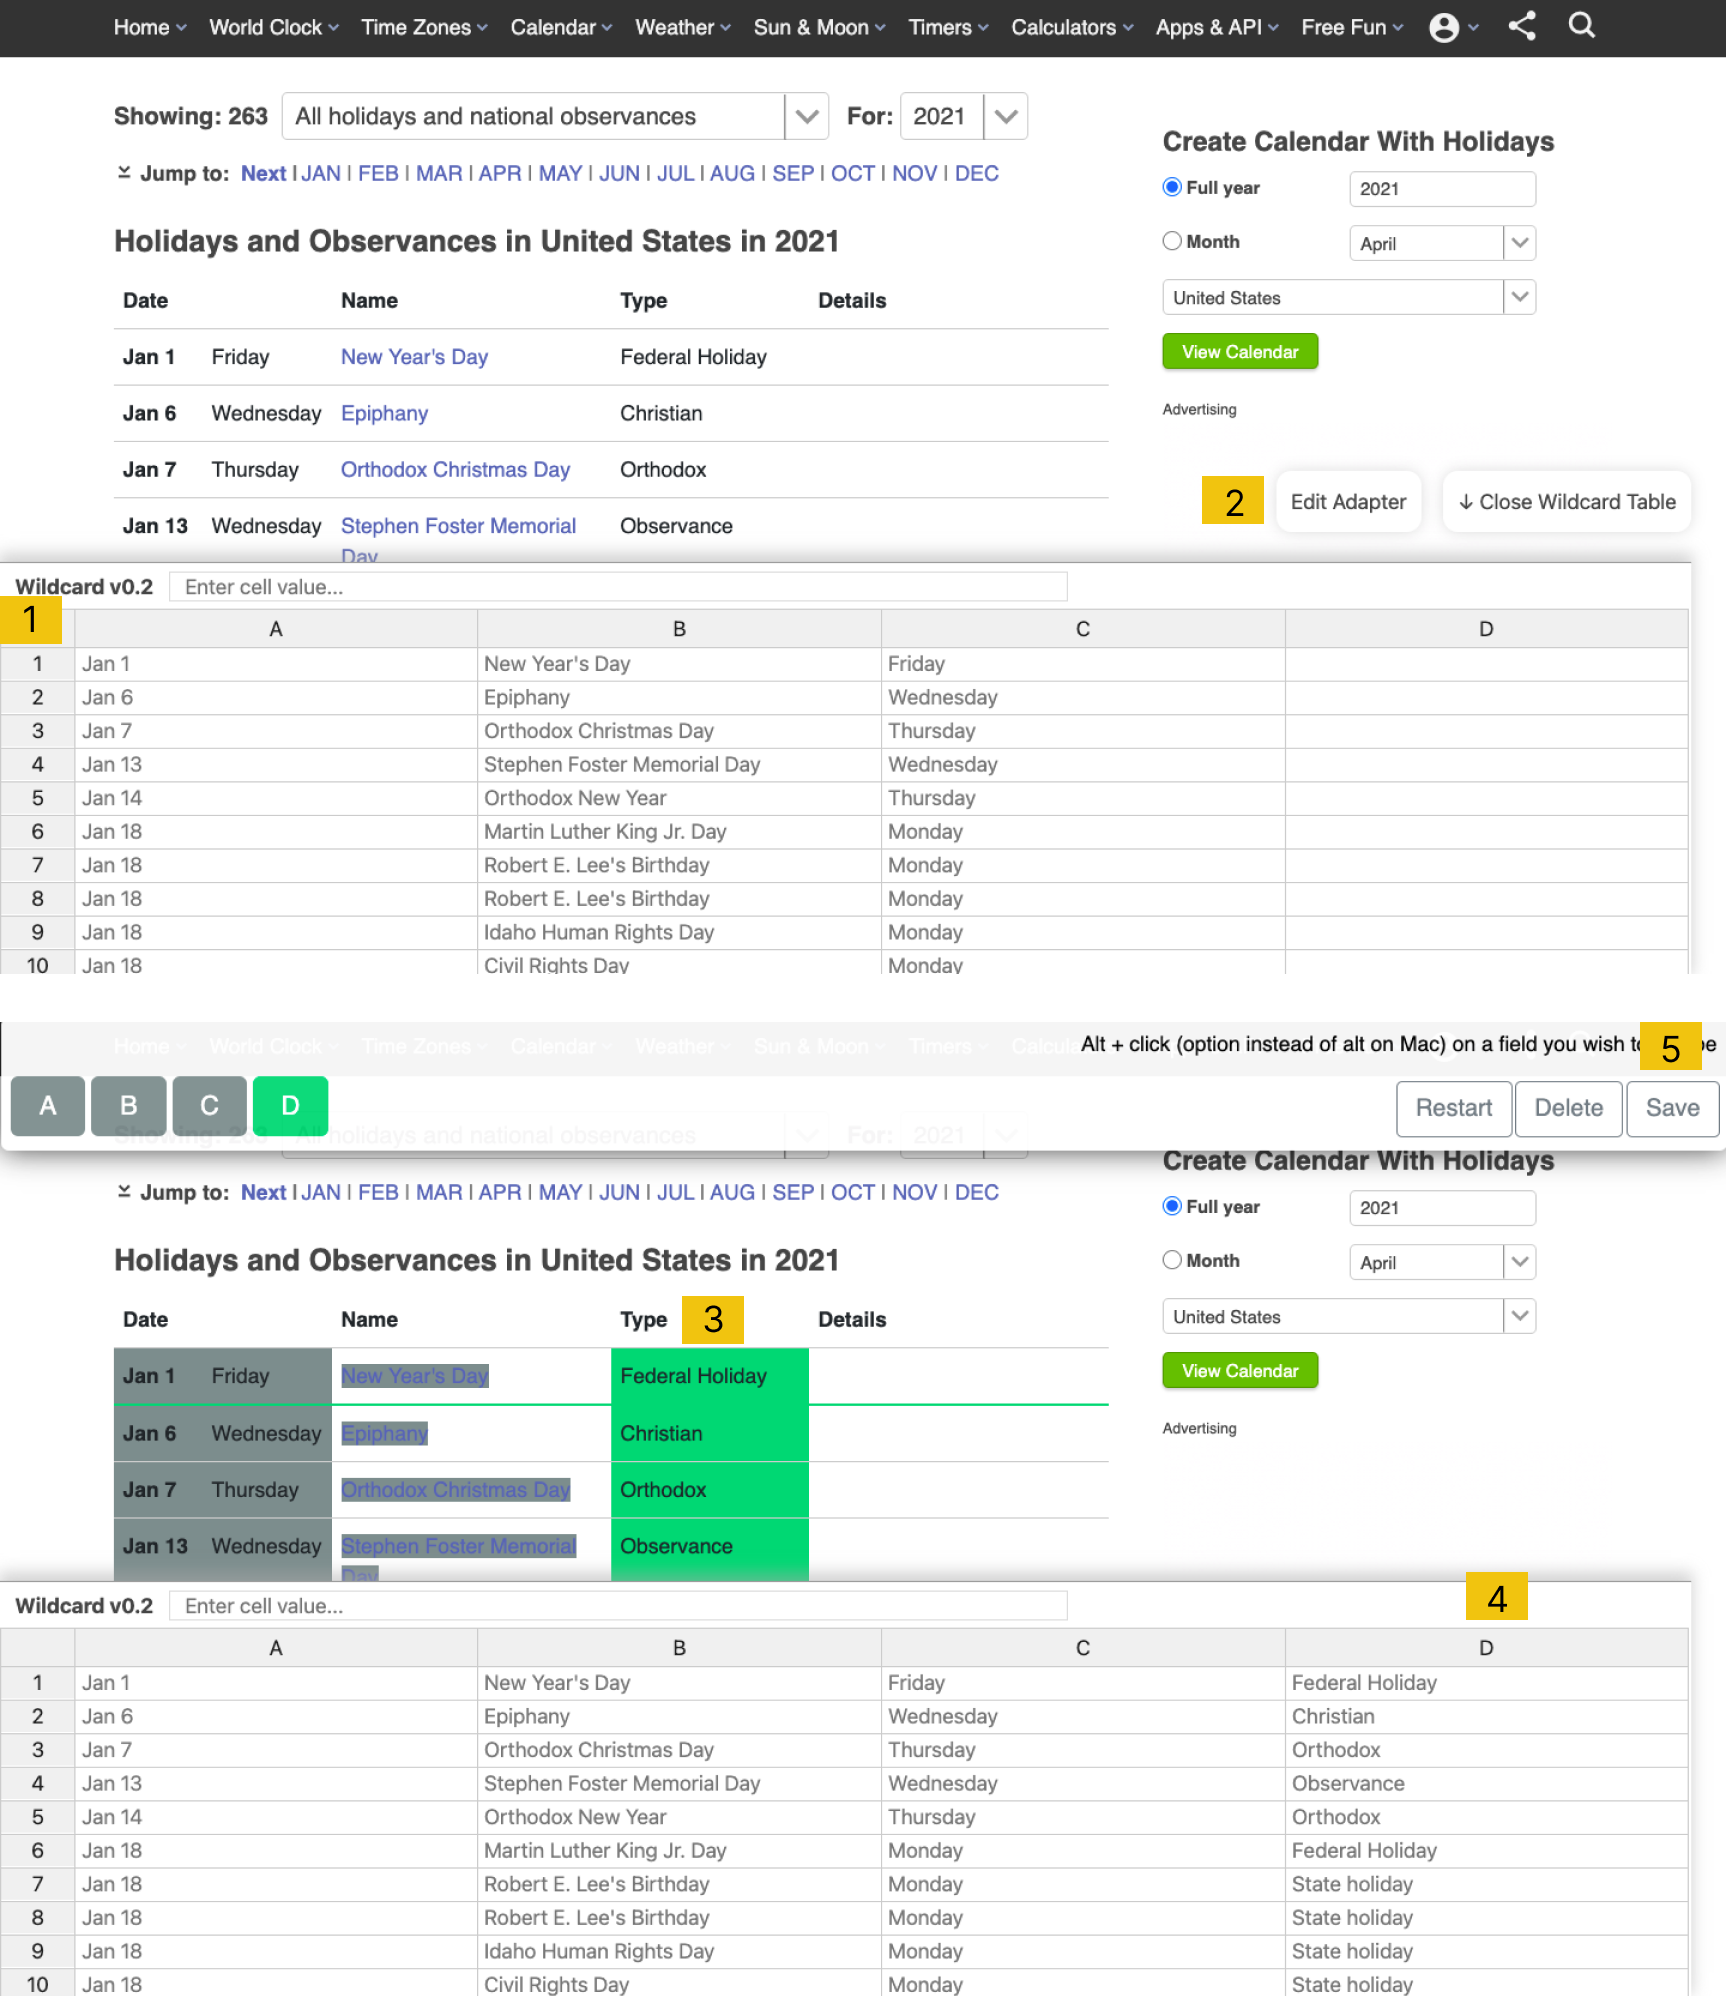
\includegraphics[width=\textwidth]{media/extending.png}
  \caption{\label{fig:extending} Extending an adapter: 1) table showing current columns and rows, 2) button for initiating adapter extension process, 3) new column value demonstrated and generalized, 4) new column values in the table and 5) button to save adapter extended by demonstration.}
\end{figure*}

The workflow is shown in Figure~\ref{fig:extending}. While viewing the
website, she clicks the ``Edit Adapter'' button (Part 2) above the
Wildcard table to initiate the adapter editing process. As she hovers
over the currently scraped values, the columns they belong to are
highlighted. Finally, she clicks on ``Federal Holiday'' (Part 3) to add
the new column of data to the table (Part 4) and saves the changes (Part
5). Jen then proceeds to sort the list by the type of holiday without
the intervention of a programmer.

\hypertarget{repairing-an-adapter}{%
\subsection{Repairing An Adapter}\label{repairing-an-adapter}}

Jen next visits Google Scholar to look up references for her thesis
project. Unfortunately, the customization she had applied to sort
publications by their title (which is not natively supported by Google
Scholar) is no longer working. In fact, the column in the Wildcard table
that contained all the publication titles is empty, because the
website's internals changed and broke the adapter's scraping logic. Jen
can repair this on her own, again taking advantage of \textbf{editing by
demonstration}.

The workflow is shown in Figure~\ref{fig:repairing}. Jen initiates the
editing process (Part 2), and initially hovers over the desired value to
demonstrate the column she wants to scrape. However, the \textbf{live
programming} interface indicates to her that the values would be
populated into column D; instead, she wants the values to be inserted
into column A where they previously appeared. So, Jen clicks on the
symbol for column A (Part 3) to indicate that she wants to scrape the
values into that column and demonstrates the first publication title
(Part 4). The missing values are now back in the table (Part 5). She
then proceeds to save her changes (Part 6) and re-apply her
customization to the website by sorting the publications by their title
without the intervention of a programmer.

\begin{figure*}
  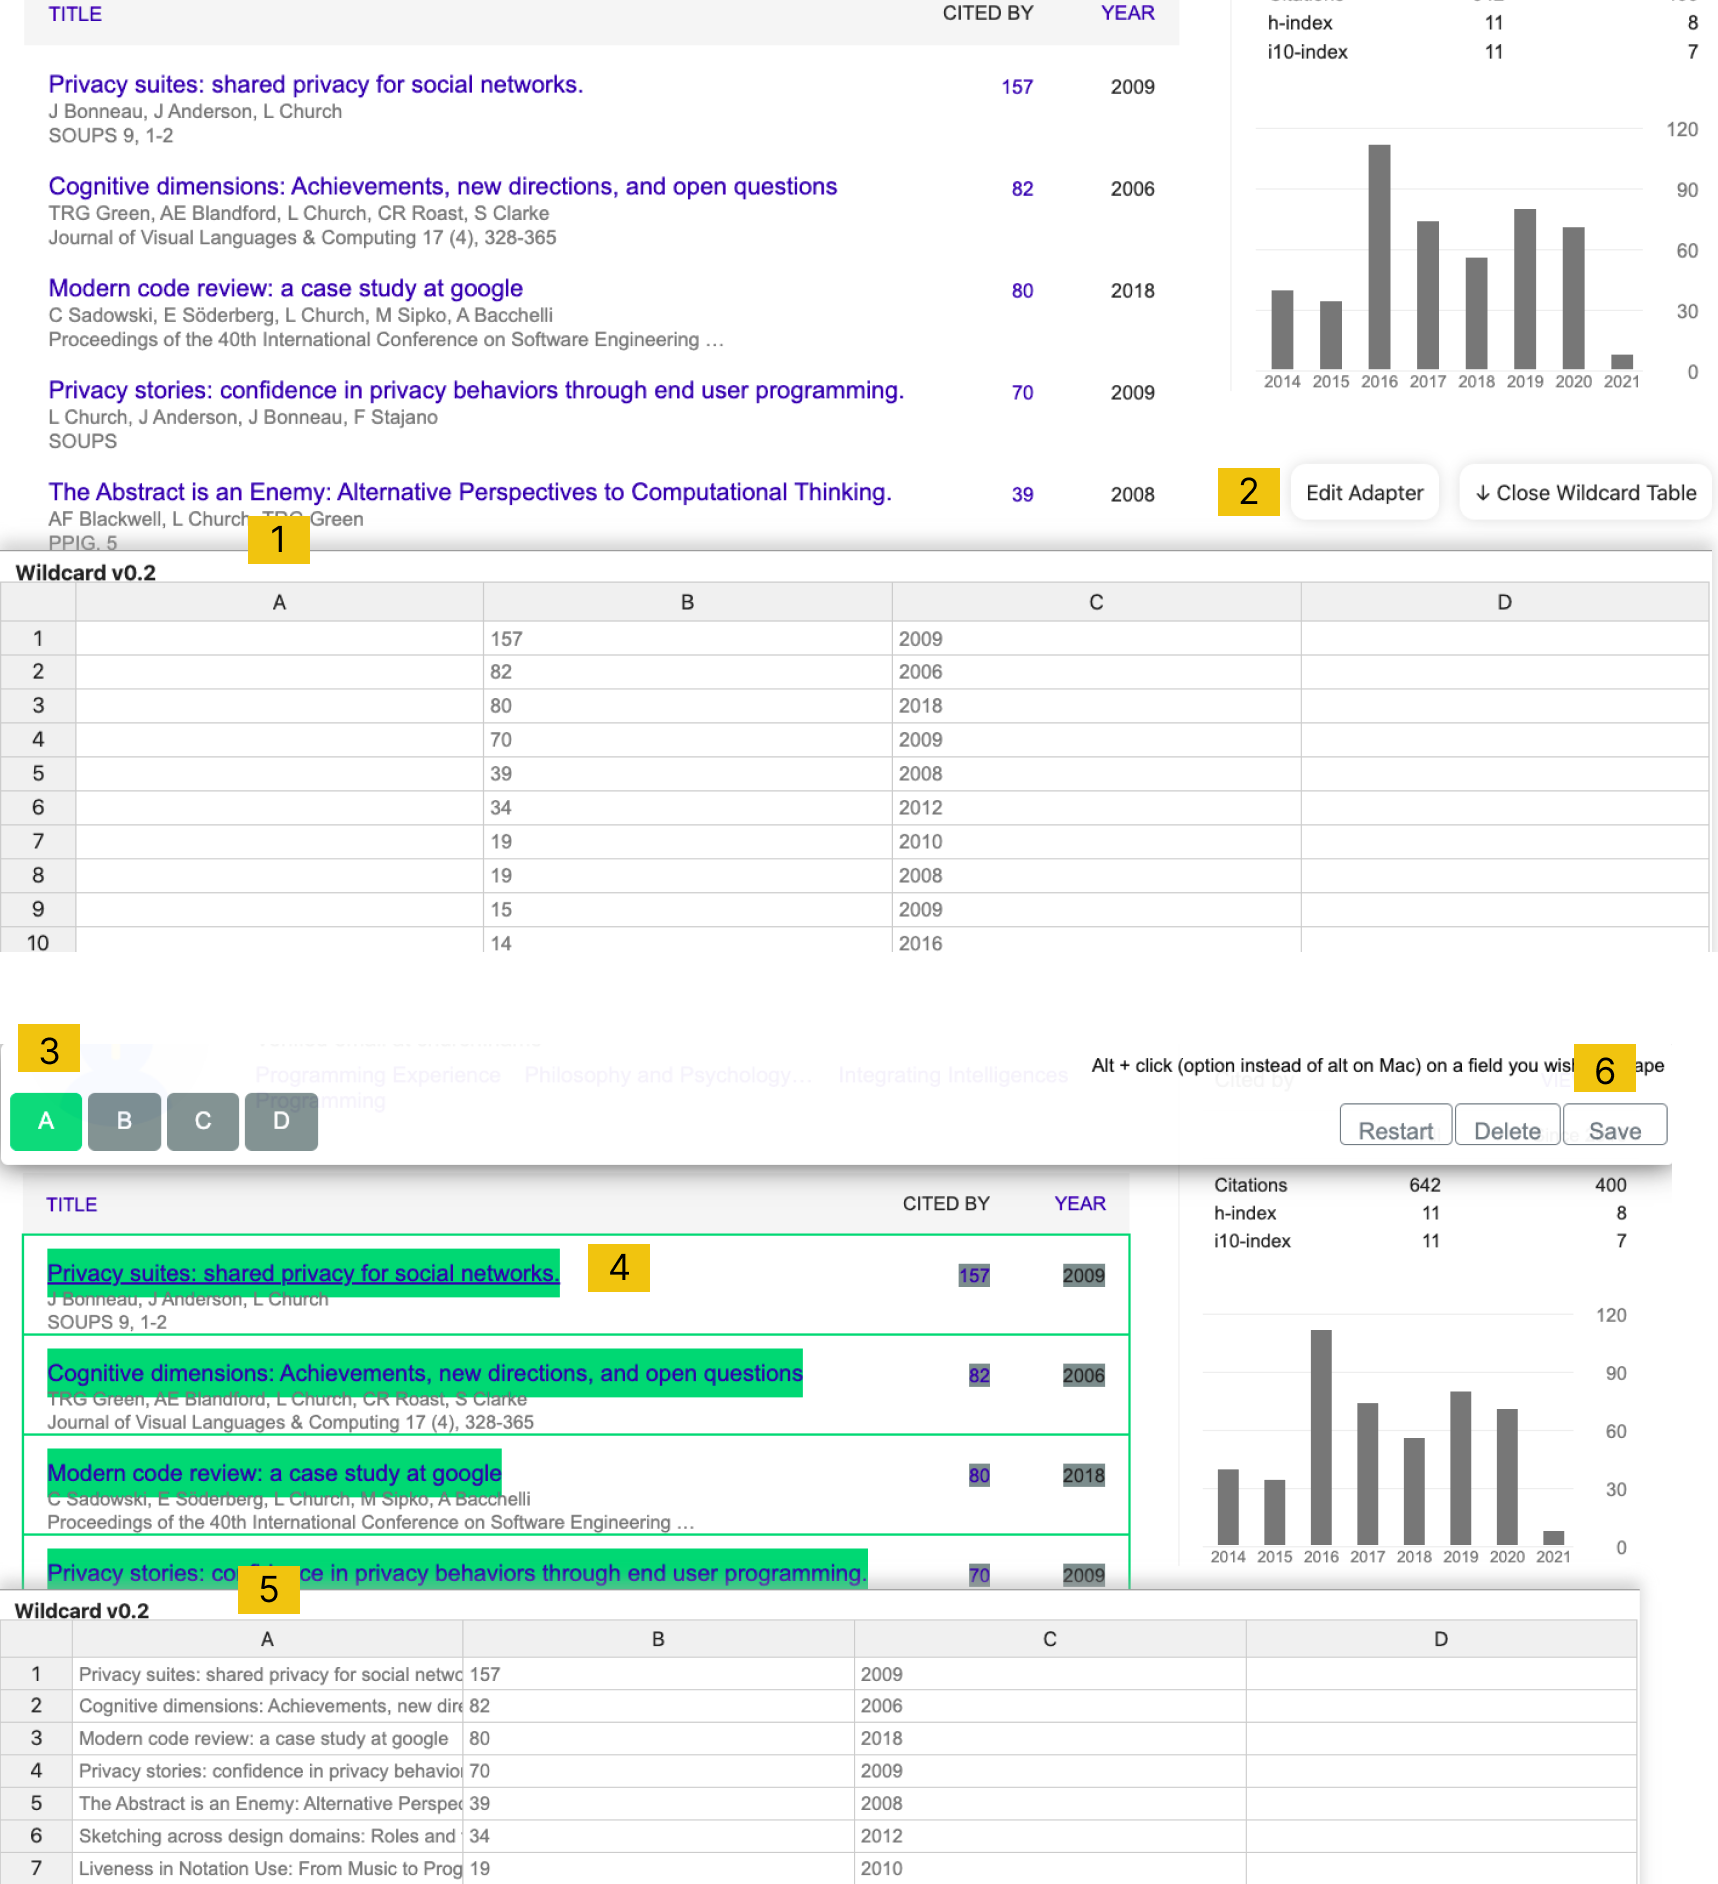
\includegraphics[width=\textwidth]{media/repairing.png}
  \caption{\label{fig:repairing} Repairing an adapter: 1) empty column in table because website changed and adapter can no longer scrape values, 2) button for initiating adapter repair 3) column to scrape data into, 4) missing column value demonstrated and generalized, 5) missing column values back in the table and 6) button to save adapter repaired by demonstration.}
\end{figure*}

\hypertarget{sec:implementation}{%
\section{System Implementation}\label{sec:implementation}}

We implemented our end-user web scraping system as an addition to the
Wildcard browser extension. We start by describing our implementations
of row and column generalization, live programming, and editing by
demonstration, and then discuss some of the current limitations of our
system.

\hypertarget{generalization-algorithms}{%
\subsection{Generalization Algorithms}\label{generalization-algorithms}}

In order to generate reusable scrapers from user demonstrations, our
system solves the \emph{wrapper induction} \citep{kushmerick2000} task:
generalizing from a small set of user-provided examples to a scraping
specification that will work on other parts of the website, and on
future versions of the website.

We take an approach similar to that used in other tools like Vegemite
\citep{lin2009} and Sifter \citep{huynh2006}:

\begin{itemize}
\tightlist
\item
  We generate a single \emph{row selector} for the website: a CSS
  selector that returns a set of Document Object Model (DOM) elements
  corresponding to individual rows of the table.
\item
  For each column in the table, we generate a \emph{column selector}, a
  CSS selector that returns the element containing the column value
  within that row.
\end{itemize}

One important difference is that our algorithm only accepts row elements
that have direct siblings with a similar structure. We refer to this as
the \emph{row-sibling} constraint. Later, we describe how the constraint
provides a useful simplification of the wrapper induction task and
discuss the resulting limitations this puts on our system.

When a user first demonstrates a column value, the generalization
algorithm is responsible for turning the demonstration into a row
selector that will correctly identify all the row elements in the
website and a column selector that will correctly identify the element
that contains the column value within a row element. During subsequent
demonstrations, the generalization algorithm uses the generated row
selector to find the row element that contains the column value and
generates a column selector which identifies the corresponding column
element.

At a high level, the generalization algorithm's challenge is to traverse
far enough up in the DOM tree from the demonstrated element to find the
element which corresponds to the row. We solve this using a heuristic;
the basic intuition is to find a large set of elements with similar
parallel structure. Consider the following sample HTML layout, which
displays a truncated table of superheroes, with each row containing some
nested structure:

\begin{figure*}
  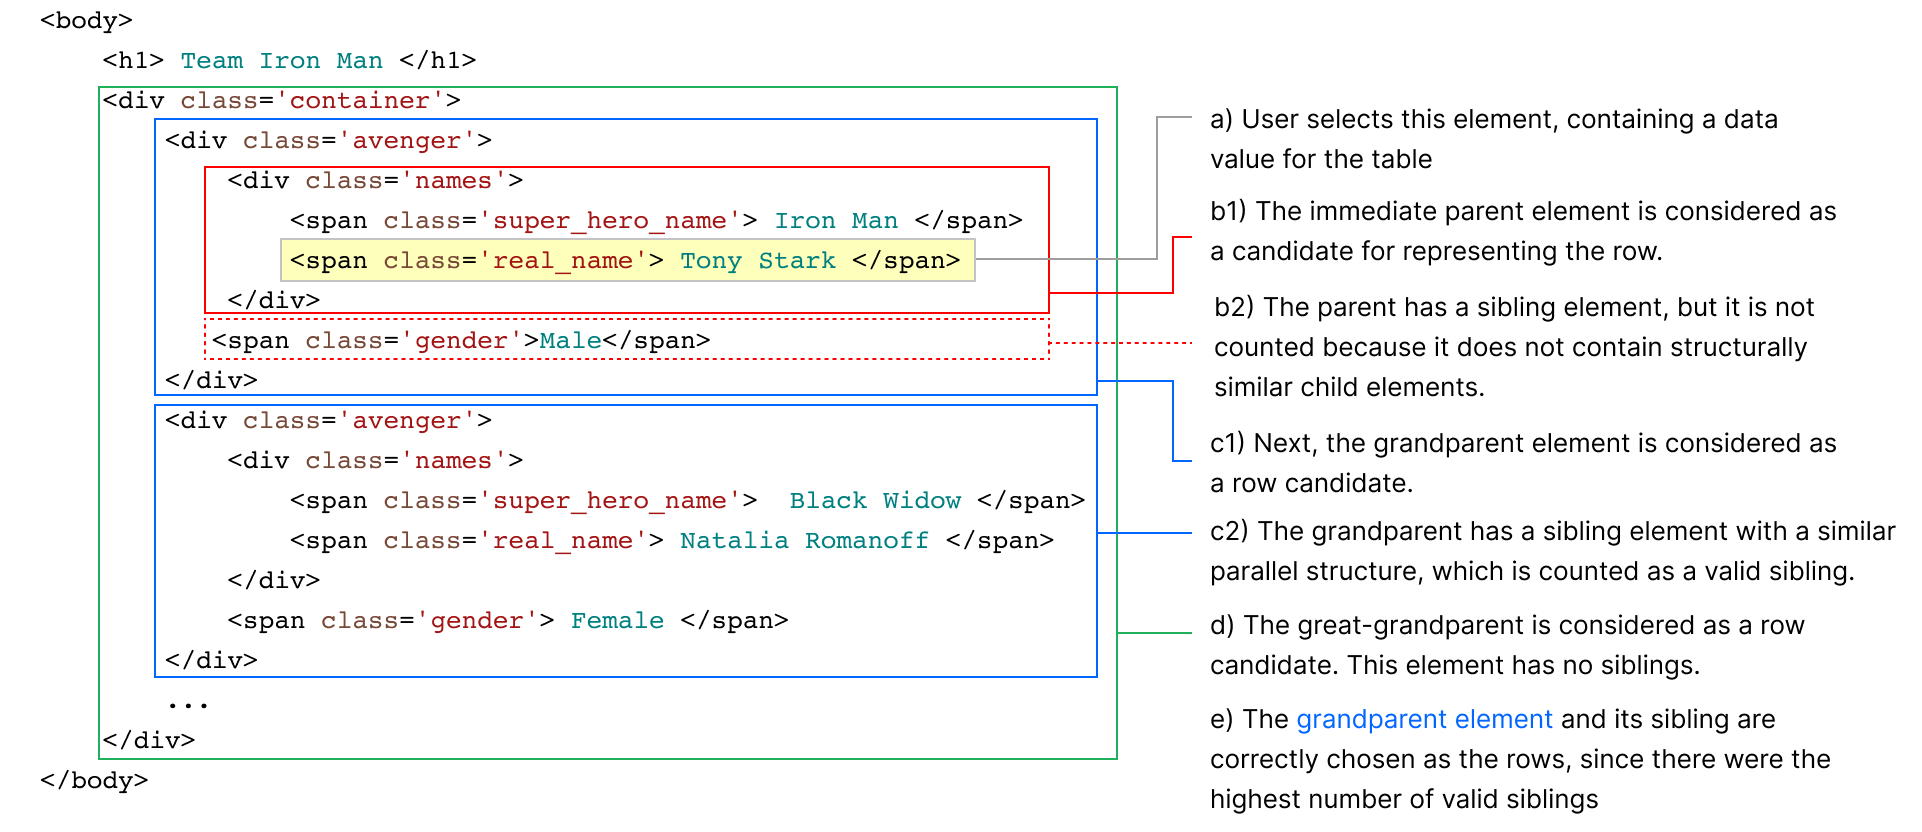
\includegraphics[width=\textwidth]{media/algorithm.png}
  \caption{\label{fig:algorithm}Our system applies a heuristic to identify DOM elements that correspond to rows in the data table.}
\end{figure*}

The user performs a demonstration by clicking on element (a) in
Figure~\ref{fig:algorithm} containing ``Tony Stark.'' Our algorithm
traverses upwards from the demonstrated element, considering each
successive parent element ((b1), (c1) and (d) in
Figure~\ref{fig:algorithm}) as a potential candidate for the row
element. For each parent element \texttt{el}, the process is as follows:

\begin{enumerate}
\def\labelenumi{\arabic{enumi}.}
\tightlist
\item
  compute a column selector \texttt{selector} that, when executed on
  \texttt{el}, only returns the demonstrated element
\item
  for each sibling \texttt{el\textquotesingle{}} of \texttt{el}, execute
  \texttt{selector} on \texttt{el\textquotesingle{}} and record whether
  the selector returns an element. If it does, this suggests that
  \texttt{el\textquotesingle{}} has some parallel structure to
  \texttt{el}.
\item
  compute \(n_{siblings}\), the number of sibling elements of
  \texttt{el} which have parallel structure.
\end{enumerate}

Notice how the \emph{row-sibling} constraint simplifies the problem. Row
candidates without siblings with parallel structure ((b1) in
Figure~\ref{fig:algorithm}) have \(n_{siblings}\) = 0, thus
disqualifying them.

The algorithm stops traversing upwards once it reaches the BODY element.
It chooses the element with the largest positive value of
\(n_{siblings}\) as the row element, preferring nodes lower in the tree
as a tiebreaker. It then generates a \emph{row selector} which returns
the row element and all its direct siblings. The column selector is the
selector that traverses from the row element to the demonstrated data
value. These row and column selectors are then used to generate a
scraping adapter which returns the DOM elements corresponding to a data
row in the table and sets up the bidirectional synchronization.

\hypertarget{live-programming}{%
\subsection{Live Programming}\label{live-programming}}

Live programming is implemented by continually running the
generalization algorithm on the DOM element under the user's cursor,
reverting if the user hovers away and committing when the user clicks.
The generated row and column selectors are used to highlight all the
matching elements on the website and create an adapter. Highlighting all
the matching column elements on the website provides visual feedback
about the system's generalization to the user. Creating an adapter
enables the system to populate the table view and set up the
bidirectional synchronization. Because the table is populated and the
bidirectional synchronization is set up, users can customize as they
scrape.

\hypertarget{editing-by-demonstration}{%
\subsection{Editing By Demonstration}\label{editing-by-demonstration}}

Our system generates adapters with the row selector and the column
selectors used to scrape the data. The row selector is a CSS selector
that identifies all the row elements of the data and the column
selectors are CSS selectors that identify each column's column elements.

When the editing process is initiated, the adapter's row selector and
column selectors are used to highlight the previously scraped values on
the website. Furthermore, the generalization algorithm takes the
adapter's row selector and uses it as the basis to generate new column
selectors after each demonstration. When a new column is demonstrated,
our system appends the generated column selector to the list of column
selectors. This is how adapters are extended to create new columns. When
an existing column is demonstrated, our system replaces the column's
current column selector with the generated column selector. This is how
adapters are repaired to fix broken columns.

Extending and repairing adapters in this manner is feasible because
column selectors are independent of each other: changing one column's
selector does not affect another column's selector. This is not the case
for system's in which the output of demonstrations are dependent on each
other. For example, in a web automation sequence that involves clicking
on a button to open a menu and then entering text into the menu's text
input, the step that enters the text is not independent because it
depends on the step that clicks the button to open the menu.

\hypertarget{limitations}{%
\subsection{Limitations}\label{limitations}}

The row-sibling constraint we mentioned earlier is important for the end
goal of customization because row elements that are not direct siblings
may not represent data on the website that should be related as part of
the same table by customizations such as sorting and filtering. In
Figure~\ref{fig:limitations} we demonstrate two examples where this
limitation becomes relevant.

\begin{figure*}
  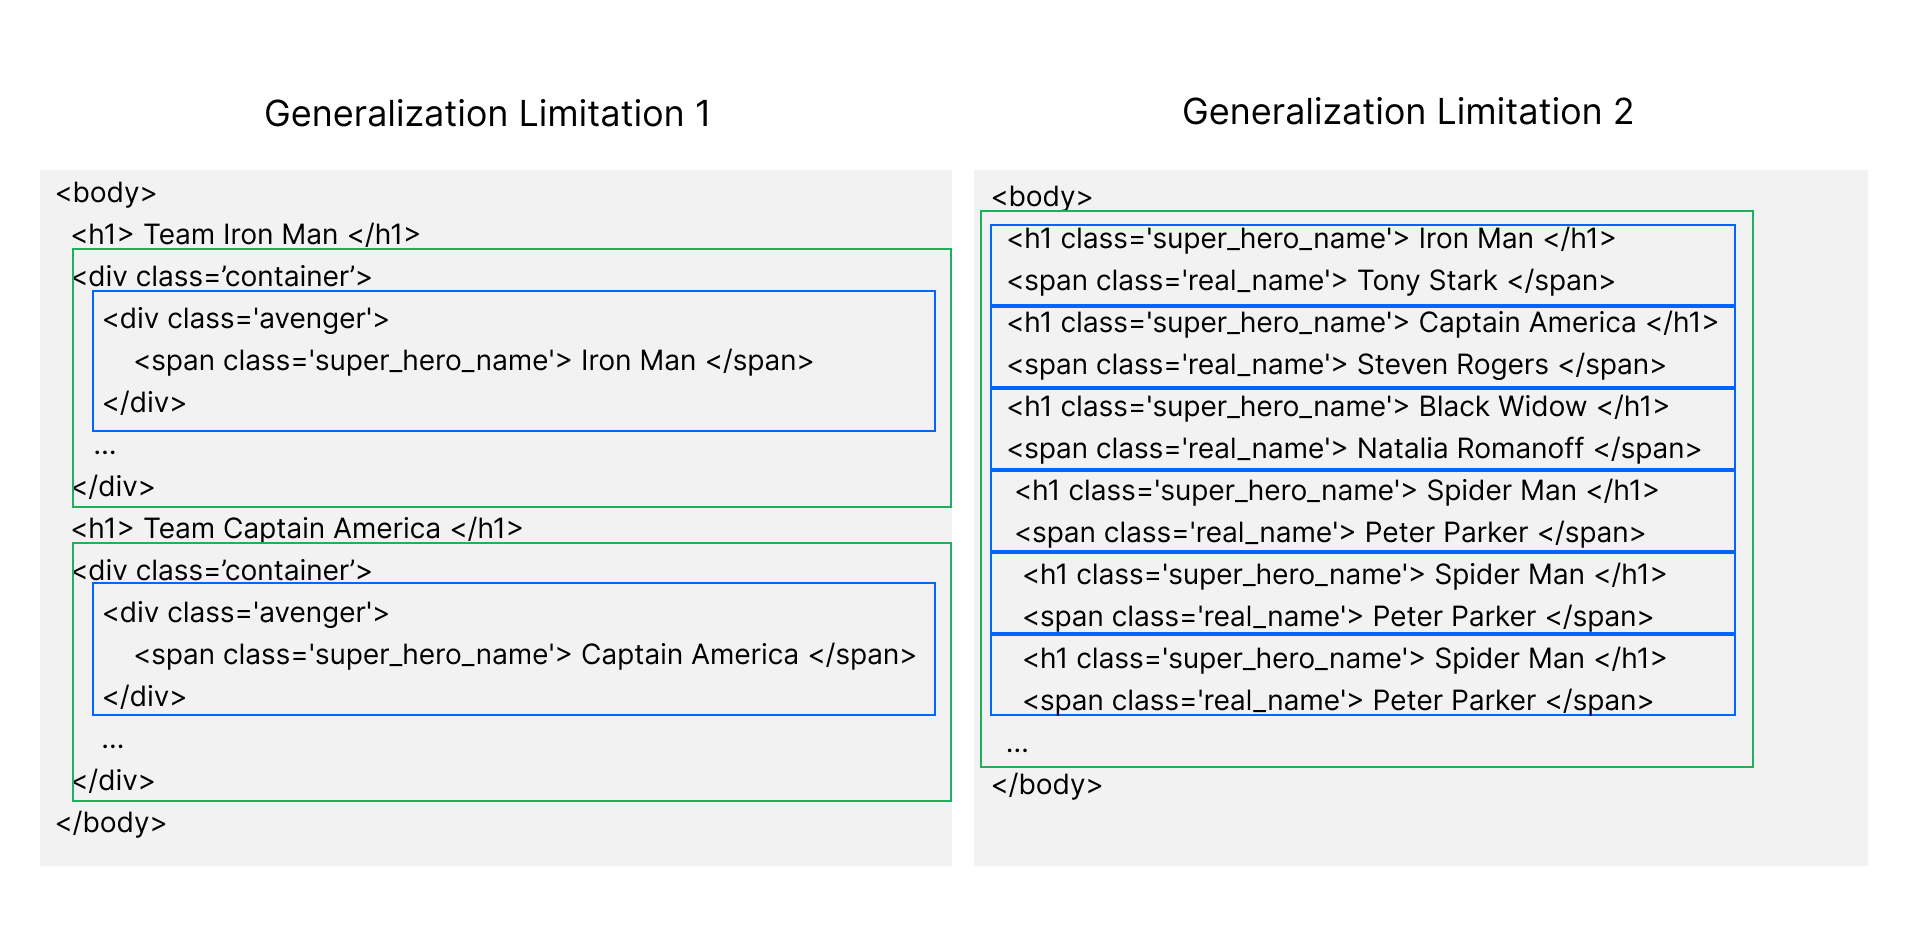
\includegraphics[width=\textwidth]{media/limitations.png}
  \caption{\label{fig:limitations} Two example pages where our generalization algorithm does not currently work. The elements with the blue border correspond to rows of the data in each layout respectively.}
\end{figure*}

\emph{Generalization Limitation 1} shows a case where the data is
displayed in a grouped structure. Without the constraint that row
elements have to be direct siblings, the row generalization algorithm
could determine the row selector to be \emph{.avenger} (elements with
blue border) because it matches the largest number of parallel
structures (has the largest \(n_{siblings}\)). While this may be the
correct result for the task of extraction, it is not necessarily
suitable for the task of customization. When the user sorts and filters,
this could result in rows moving between the two tables, disrupting the
nested layout and producing a confusing result. Because of this, our
system currently does not support such layouts. In the future, we may
explore the possibility of extracting multiple tables from a website and
joining them together.

\emph{Generalization Limitation 2}, also in
Figure~\ref{fig:limitations}, shows a case where the website contains
one table of data in which rows are made up of alternating H1 and SPAN
tags (elements with blue border). This poses a challenge because each
row does not correspond directly to a single DOM element; instead, each
row consists of multiple consecutive DOM elements without any grouped
structure. Moving the rows when customizing the webpage would require
treating multiple consecutive elements as a single row. This is
supported in the underlying Wildcard system, but not yet by our tool.

Our system also does not support scraping data loaded after the initial
websites render as the user scrolls. Site adapters hand-coded in
Javascript can specify event listeners on the DOM to re-execute the
scraping code when new data is loaded as a user scrolls. In future work,
we plan to provide a mechanism for end-users to specify when a
demonstrated adapter should re-execute its scraping code in response to
user scrolling. We also do not support scraping data across multiple
pages of related data, but this context poses more fundamental
challenges to the idea of web customization, since users would somehow
need to perform customizations across multiple pages in coordination.

\hypertarget{sec:design-principles}{%
\section{Design Principles}\label{sec:design-principles}}

Below, we discuss the three design principles underlying our work and
how they relate to the broader field of end-user web scraping and
customization.

\hypertarget{unified-environment}{%
\subsection{Unified Environment}\label{unified-environment}}

In the previous iteration of Wildcard, web scraping was an entirely
separate activity from customization. Programmers that wrote scraping
adapters would need to switch into an IDE to write code as part of
customizing a new website.

This type of divide between tasks appears in other domains. In data
science, workflows revolve between cleaning and using data but this
often happens in different environments. The creators of Wrex
\citep{drosos2020}, an end-user programming-by-example system for data
wrangling, reported that ``although data scientists were aware of and
appreciated the productivity benefits of existing data wrangling tools,
having to leave their native notebook environment to perform wrangling
limited the usefulness of these tools.'' This was a major reason Wrex
was developed as an add-on to Jupyter notebooks, the environment in
which data scientists use their data. In web scraping, if a user comes
across an omission while working with data scraped from a website, they
need to switch from the environment in which they are using the data to
the environment in which they created their scraping code in order to
edit and re-run it. This can be seen in many end-user web scraping
systems like Rousillon \citep{chasins2018}and FlashExtract
\citep{le2014} and commercial tools like import.io \citep{import.io},
dexi.io \citep{dexi.io}, Octoparse \citep{octoparse} and ParseHub
\citep{parsehub}. In web customization, the creators of Vegemite
\citep{lin2009}, a system for end-user programming of mashups, reported
that participants of its user study thought ``it was confusing to use
one technique to create the initial table, and another technique to add
information to a new column.'' This hints at the need for both a unified
environment and a unified workflow.

In this work, we have combined scraping and customization into a single,
unified environment with a unified workflow. The goal is to minimize the
environment switch between \emph{extracting} the data and \emph{using}
the data. A user might start out by scraping some data on a website, and
then switch to customizing the website using the results. Then, they
might realize they need more data to perform their desired task, at
which point they can easily extend the adapter by demonstrating new
columns. All of these tasks take place right in the browser, where the
user was initially already using the website. Instead of bringing the
data to another tool, we have brought a tool to the data. This directly
relates to the idea of ``in-place toolchains'' \citep{zotero-1362} being
an integral part of end-user programming systems.

Of course, there is value in specialized tools: Wildcard has nowhere
near the full capabilities of spreadsheet software or databases.
Nevertheless, we believe a single, unified environment for scraping and
customization presents a significantly lower barrier to entry for
customization.

\hypertarget{editing-by-demonstration-1}{%
\subsection{Editing By Demonstration}\label{editing-by-demonstration-1}}

Many end-user web scraping and macro systems allow users to
\emph{create} programs by demonstration but do not offer a way to
\emph{edit} them by demonstration. In Rousillon \citep{chasins2018}, a
web scraping program created by demonstration can only be edited through
a high-level, block-based programming language called Helena
\citep{zotero-1349}. Helena supports adding control flow logic
(conditional execution, wait times etc) which is invaluable for
automating access to websites. However, it does not support extending
the web scraping code to add new columns after the demonstration or
repairing it to provide new selectors if the website changes. In
Vegemite \citep{lin2009}, a web automation program created through
demonstration can only be edited by editing the text-based
representation of the automation demonstrations. In fact, only the
demonstrations used to perform automations on the scraped website data
can be edited. If a user needs to add a new column or repair an existing
one in the scraped data table, they need to re-demonstrate the columns
and then re-run the automation script. One exception to existing editing
models worth pointing out is import.io \citep{import.io}. It allows
users to add new columns by demonstration but it is not clear whether
deleting a column and re-demonstrating it could serve the purpose of
repair.

In Wildcard, if a website's hand-coded adapter ceases to function
because the website changes, the table may lose its data which means
that an end-user's customizations may also cease to function.
Furthermore, end-users are powerless to extend the scraping adapter to
add columns to the table in order to perform new customizations. This
goes against MacLean et. al.'s vision of user-tailorable systems
\citep{maclean1990} that give users ``a feeling of ownership of the
system, to feel in control of changing the system and to understand what
can be changed.'' Providing an easy way for users to edit programs is
therefore fundamental to fully democratizing web customization.

Editing by demonstration makes end-users first-class citizens in the
customization ecosystem. Because users interact with the scraped data
through a unified environment directly in the context of the website, it
is easy to initiate the scraping system in editing mode: the scraping
system is simply booted up using metadata stored with the scraping
adapter to the state when the demonstration was completed. Users that
have gone through the creation process will immediately realize what to
do in order to extend or repair the adapter. Users that have not gone
through the creation process might have a harder time but we provide
visual clues (such as highlighting the row to perform demonstrations
from with a green border) and live programming (immediately preview the
results of demonstrations) that serve as guides.

As discussed in Section~\ref{sec:implementation}, editing by
demonstration in the web scraping domain is feasible because column
selectors are independent of each other. However, this is not the case
with row selectors because column selectors are dependent on them. Our
system therefore does not support editing rows but this an acceptable
limitation given our focus on extension and repair which only involve
column selectors.

\hypertarget{live-programming-1}{%
\subsection{Live Programming}\label{live-programming-1}}

In many programming-by-demonstration web scraping systems
\citep[\citet{lin2009}]{chasins2018}, users only get \emph{full}
feedback about the program's execution (generalization and the scraped
values) after providing \emph{all} the demonstrations. This means they
cannot adjust their demonstrations in response to the system's feedback
as they demonstrate.

Our end-user web scraping system employs live programming techniques to
eliminate this edit-compile-debug cycle by running the generalization
algorithm and generating an adapter after each user demonstration. As we
showed in Section~\ref{sec:demos}, when a user demonstrates a value of a
column they wish to scrape, our system immediately shows how it has
generalized the user's demonstration across the other rows of the data
by highlighting the all relevant values. It also populates the table
with the scraped data based on the latest demonstration. The
highlighting and table population serve to give users a view of how
their demonstration has been generalized and what data will be available
in the table once scraped.

Many successful end-user programming systems such as spreadsheets and
SQL provide users with immediate results after entering commands. Our
live programming environment is particularly similar to that of
FlashProg \citep{mayer2015}, a framework that provides user interface
support for programming-by-demonstration systems like FlashExtract
\citep{le2014}, and relates to the idea that an important quality of
end-user programming is ``interaction with a living system''
\citep{zotero-1362}.

Unlike text-based commands which are only valid once complete (e.g
\texttt{SELECT\ *\ FRO} versus \texttt{SELECT\ *\ FROM\ user\_table}),
the target of demonstration commands (the value of a DOM element under
the cursor) is the same during both hover and click (incomplete command
versus complete command). This allows us to take a small step further by
executing a command before a user completes it, thereby providing them
with a preview of the results on hover.

There are limits to this approach. Providing live feedback on websites
with a large number of DOM elements or complex CSS selectors can slow
down the generalization process, especially if a user is constantly
moving their cursor. Furthermore, many datasets are too large to preview
in the table in their entirety; the user might benefit more from the
live feedback if it could summarize large datasets. For example,
FlashProg provides a summary of the generalization through a color-coded
minimap next to the scrollbar of its extraction interface.

\hypertarget{sec:related-work}{%
\section{Related Work}\label{sec:related-work}}

End-user web scraping for customization relates to existing work in
end-user web scraping by a number of tools.

FlashProg \citep{mayer2015} is a framework that provides user interface
support for FlashExtract \citep{le2014}, a framework for data scraping
by examples. FlashProg's interface provides immediate visual feedback
about the generalization and scrapes the matched values into an output
tab. In addition, it has a program viewer tab that contains a high level
description of what the generated program is doing and provides a list
of alternative programs. Finally, it has a disambiguation tab that
utilizes conversational clarification to disambiguate programs, the
conservations with the user serving as inputs to generate better
programs. Though FlashProg has many desirable features we aim to
implement in future iterations, its implementation does not align with
our goal to provide a unified environment within a browser for scraping
and customizing websites.

Rousillon \citep{chasins2018} is a tool that enables end-users to scrape
distributed, hierarchical web data. Because demonstrations can span
across several websites and involve complex data access automation
tasks, its interface does not provide \emph{full} live feedback about
its generalizations or the values to be scrapped until all the
demonstrations have been provided and the generated program has been
run. If run on a website it has encountered before, Rousillon makes all
the previously determined generalizations visible to the user by
color-coding the values on the website that belong to the same column.
This is a desirable feature for our system as users will not have to
actively explore in order to discover which values are available for
scraping and how they are related to each other. On the extension and
repair front, Rousillon presents the web scraping code generated by
demonstration as an editable, high-level, block-based language called
Helena \citep{zotero-1349}. While Helena can be used to perform more
complex editing tasks like adding control flow, it does not support
adding or repairing columns after the demonstrations and presents a
change in the model used for creation. Our system maintains the model
used for creation by allowing users to extend and repair web scraping
code via demonstration.

Vegemite \citep{lin2009} is a tool for end-user programming of mashups.
It has two interfaces: one for scraping values from a website and
another for creating scripts that operate on the scraped values. The web
scraping interface does not provide live feedback about the
generalization on hover but after a user clicks a value, the interface
shows the result of the system's generalization by highlighting the all
matched values. Furthermore, even though the interface also has a table,
the table is only populated with the scraped values after all the
demonstrations have been provided. The scripting interface utilizes
CoScripter \citep{leshed2008} which is used to record operations on the
scraped values for automation. For example, the scripting interface can
be used to demonstrate the task of copying an address in the table,
pasting it into a walk score calculator and pasting the result back into
the table. The script would then be generalized to all the rows and
re-run to fill in the remaining walk scores. CoScripter provides the
generated automation program as text-based commands, such as ``paste
address into `Walk Score' input,'' which can be edited after the program
is created via ``sloppy programming'' \citep{lin2009} techniques.
However, this editing does not extend to the web scraping interface used
for demonstrations and presents a change in the model used for creation.

Sifter \citep{huynh2006} is a tool that augments well structured
websites with advanced sorting and filtering functionality. Like
Wildcard, it uses web scraping to extract data from websites in order to
enable customizations (sorting and filtering). Unlike Wildcard, it does
not support adding annotations to websites and running computations on
the scraped data using a spreadsheet formula language. Both of these
significantly expand the types of customizations end-users can make to
websites. Sifter performs the web scraping automatically using a variety
of heuristics and solicits guidance from the user if this fails. While
automatic web scraping seems desirable, it is unclear how useful it is
if the goal is customization. Given a row with ten scrapable values, and
therefore ten columns, would a user prefer to simply demonstrate the
value for the single column they are interested in or un-demonstrate the
nine values they are not interested in? This automatic web scraping
approach can be also be seen in tools like import.io \citep{import.io}
so it is certainly worth evaluating as part of a user study.

\hypertarget{sec:conclusion}{%
\section{Conclusion And Future Work}\label{sec:conclusion}}

In this paper, we presented our progress towards \emph{end-user web
scraping for customization}, to empower end-users in Wildcard's
ecosystem to create, extend and repair scraping adapters. There are
several outstanding issues and open questions we hope to address in
future work.

Like existing programming-by-demonstration approaches, web scraping in
our current implementation is limited to what can be demonstrated. This
is problematic if users want to scrape the URL associated with a link
element, which is not visible, or only scrape a substring of a value. To
solve this, we plan to harness Wildcard's formula language. End-users
will be able to use formulas targeted at web scraping to access DOM
element properties and attributes. For example, a formula like
\texttt{=GetAttribute(link\_column,\ ‘href’)} could be used to scrape
URLs of link elements. End-users will also be able to use formulas
targeted at data processing. For example, a formula like
\texttt{=GetSubstring(name\_column,\ 1,\ 2)} could be used to scrape
substrings of text values. Such web scraping and data processing
formulas will give end-users some of the power available to programmers
that write web scraping code in Javascript which supports a wide variety
of DOM access and processing ability.

To assess our design principles, we plan to carry out a broader
evaluation of our system through a user study. So far, we have only
tested the system amongst ourselves and a small number of colleagues.
More testing is needed to understand whether it can be successfully used
among a broader set set of users across a wider variety of websites.
Furthermore, we plan to incorporate the program viewer and
disambiguation features of FlashProg \citep{mayer2015} to give users
more insight and control into the generalization process.

Our end goal is to empower end-users to customize websites in an
intuitive and flexible way, and thus make the web more malleable for all
of its users.

% \printbibliography

%%
%% The next two lines define the bibliography style to be used, and
%% the bibliography file.
\bibliographystyle{ACM-Reference-Format}
\bibliography{references.bib}

\end{document}
\endinput
%%
%% End of file `sample-sigconf.tex'.
